\documentclass{standalone}
\usepackage{tikz}
\usetikzlibrary{patterns, positioning}


\begin{document}
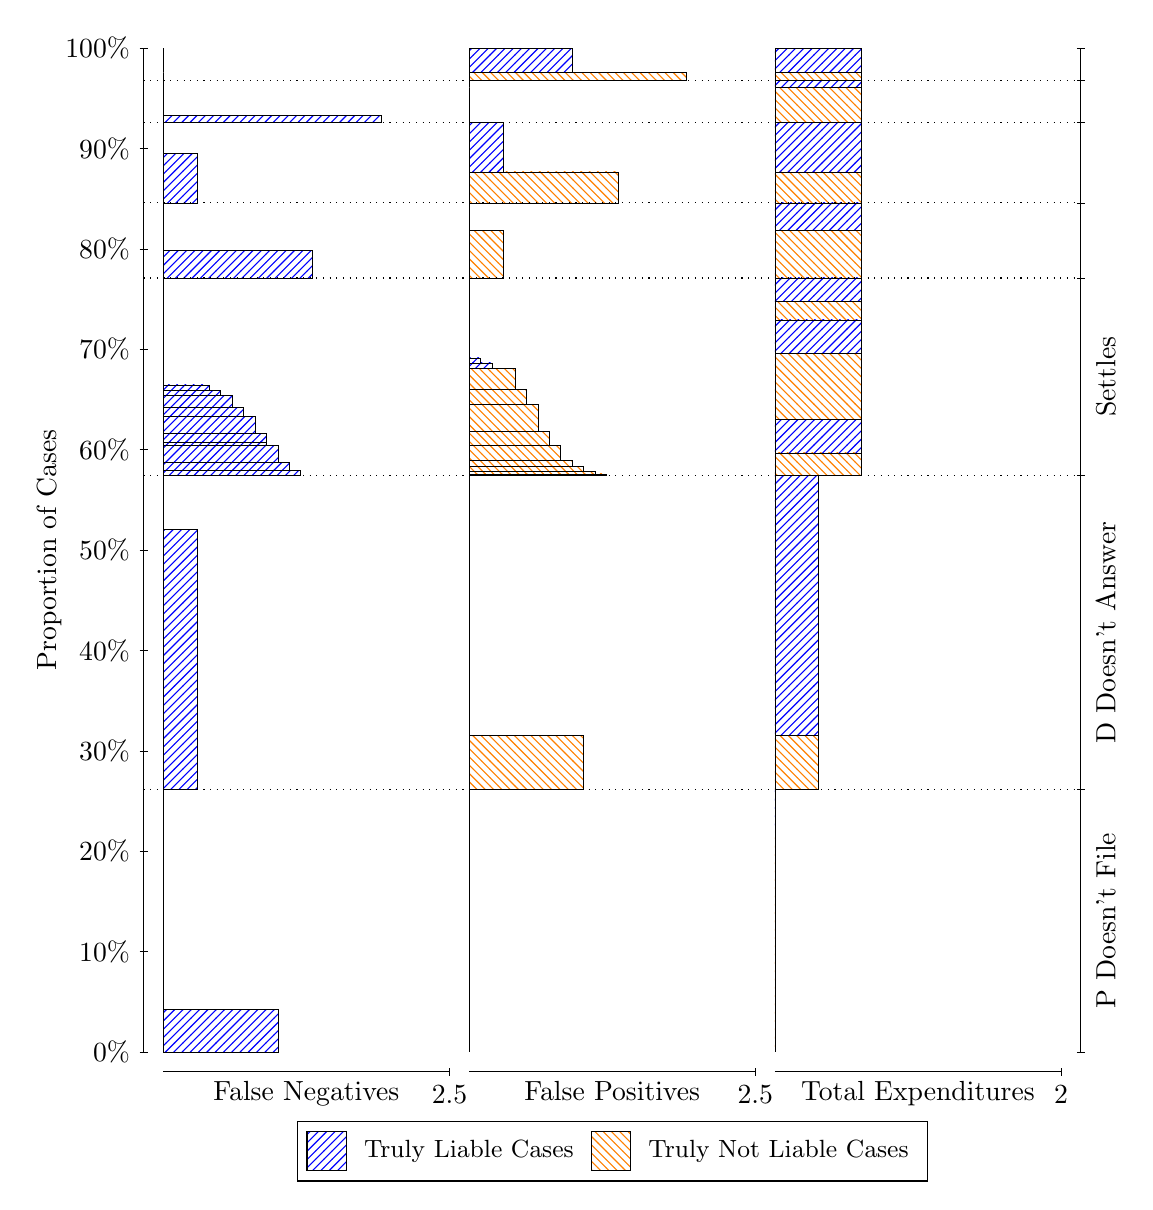
\begin{tikzpicture}
\draw[black, very thin] (1.5,1.75) -- (1.5,14.5);
\node[rotate=90, text=black, anchor=center] at (0.3, 8.125) {Proportion of Cases};
\draw[black, very thin] (1.45,1.75) -- (1.55,1.75);
\node[text=black, anchor=east] at (1.45, 1.75) {0\%};
\draw[black, very thin] (1.45,3.025) -- (1.55,3.025);
\node[text=black, anchor=east] at (1.45, 3.025) {10\%};
\draw[black, very thin] (1.45,4.3) -- (1.55,4.3);
\node[text=black, anchor=east] at (1.45, 4.3) {20\%};
\draw[black, very thin] (1.45,5.575) -- (1.55,5.575);
\node[text=black, anchor=east] at (1.45, 5.575) {30\%};
\draw[black, very thin] (1.45,6.85) -- (1.55,6.85);
\node[text=black, anchor=east] at (1.45, 6.85) {40\%};
\draw[black, very thin] (1.45,8.125) -- (1.55,8.125);
\node[text=black, anchor=east] at (1.45, 8.125) {50\%};
\draw[black, very thin] (1.45,9.4) -- (1.55,9.4);
\node[text=black, anchor=east] at (1.45, 9.4) {60\%};
\draw[black, very thin] (1.45,10.675) -- (1.55,10.675);
\node[text=black, anchor=east] at (1.45, 10.675) {70\%};
\draw[black, very thin] (1.45,11.95) -- (1.55,11.95);
\node[text=black, anchor=east] at (1.45, 11.95) {80\%};
\draw[black, very thin] (1.45,13.225) -- (1.55,13.225);
\node[text=black, anchor=east] at (1.45, 13.225) {90\%};
\draw[black, very thin] (1.45,14.5) -- (1.55,14.5);
\node[text=black, anchor=east] at (1.45, 14.5) {100\%};

\draw[black, very thin] (13.4,1.75) -- (13.4,14.5);
\draw[black, very thin] (13.35,1.75) -- (13.45,1.75);
\node[anchor=west] at (13.35, 1.75) {};
\draw[black, very thin] (13.35,5.081) -- (13.45,5.081);
\node[anchor=west] at (13.35, 5.081) {};
\draw[black, very thin] (13.35,9.0697) -- (13.45,9.0697);
\node[anchor=west] at (13.35, 9.0697) {};
\draw[black, very thin] (13.35,11.58) -- (13.45,11.58);
\node[anchor=west] at (13.35, 11.58) {};
\draw[black, very thin] (13.35,12.534) -- (13.45,12.534);
\node[anchor=west] at (13.35, 12.534) {};
\draw[black, very thin] (13.35,13.553) -- (13.45,13.553);
\node[anchor=west] at (13.35, 13.553) {};
\draw[black, very thin] (13.35,14.092) -- (13.45,14.092);
\node[anchor=west] at (13.35, 14.092) {};
\draw[black, very thin] (13.35,14.5) -- (13.45,14.5);
\node[anchor=west] at (13.35, 14.5) {};

\draw[black, very thin, pattern color=blue, pattern=north east lines] (1.75,1.75) rectangle (3.2033,2.2902);
\draw[black, very thin, pattern color=orange, pattern=north west lines] (1.75,2.2902) rectangle (1.75,5.081);
\draw[black, very thin, pattern color=blue, pattern=north east lines] (1.75,5.081) rectangle (2.186,8.3827);
\draw[black, very thin, pattern color=orange, pattern=north west lines] (1.75,8.3827) rectangle (1.75,9.0697);
\draw[black, very thin, pattern color=blue, pattern=north east lines] (1.75,9.0697) rectangle (3.494,9.1404);
\draw[black, very thin, pattern color=blue, pattern=north east lines] (1.75,9.1404) rectangle (3.3487,9.241);
\draw[black, very thin, pattern color=blue, pattern=north east lines] (1.75,9.241) rectangle (3.2033,9.4567);
\draw[black, very thin, pattern color=blue, pattern=north east lines] (1.75,9.4567) rectangle (3.058,9.4977);
\draw[black, very thin, pattern color=blue, pattern=north east lines] (1.75,9.4977) rectangle (3.058,9.6067);
\draw[black, very thin, pattern color=blue, pattern=north east lines] (1.75,9.6067) rectangle (2.9127,9.8195);
\draw[black, very thin, pattern color=blue, pattern=north east lines] (1.75,9.8195) rectangle (2.7673,9.9327);
\draw[black, very thin, pattern color=blue, pattern=north east lines] (1.75,9.9327) rectangle (2.622,10.085);
\draw[black, very thin, pattern color=blue, pattern=north east lines] (1.75,10.085) rectangle (2.4767,10.148);
\draw[black, very thin, pattern color=blue, pattern=north east lines] (1.75,10.148) rectangle (2.3313,10.221);
\draw[black, very thin, pattern color=orange, pattern=north west lines] (1.75,10.221) rectangle (1.75,11.58);
\draw[black, very thin, pattern color=blue, pattern=north east lines] (1.75,11.58) rectangle (3.6393,11.927);
\draw[black, very thin, pattern color=orange, pattern=north west lines] (1.75,11.927) rectangle (1.75,12.534);
\draw[black, very thin, pattern color=blue, pattern=north east lines] (1.75,12.534) rectangle (2.186,13.159);
\draw[black, very thin, pattern color=orange, pattern=north west lines] (1.75,13.159) rectangle (1.75,13.553);
\draw[black, very thin, pattern color=blue, pattern=north east lines] (1.75,13.553) rectangle (4.5113,13.649);
\draw[black, very thin, pattern color=orange, pattern=north west lines] (1.75,13.649) rectangle (1.75,14.092);
\draw[black, very thin, pattern color=orange, pattern=north west lines] (1.75,14.092) rectangle (1.75,14.188);
\draw[black, very thin, pattern color=blue, pattern=north east lines] (1.75,14.188) rectangle (1.75,14.5);
\draw[black, very thin, pattern color=orange, pattern=north west lines] (5.6333,1.75) rectangle (5.6333,4.5408);
\draw[black, very thin, pattern color=blue, pattern=north east lines] (5.6333,4.5408) rectangle (5.6333,5.081);
\draw[black, very thin, pattern color=orange, pattern=north west lines] (5.6333,5.081) rectangle (7.0867,5.768);
\draw[black, very thin, pattern color=blue, pattern=north east lines] (5.6333,5.768) rectangle (5.6333,9.0697);
\draw[black, very thin, pattern color=orange, pattern=north west lines] (5.6333,9.0697) rectangle (7.3773,9.0914);
\draw[black, very thin, pattern color=orange, pattern=north west lines] (5.6333,9.0914) rectangle (7.232,9.1185);
\draw[black, very thin, pattern color=orange, pattern=north west lines] (5.6333,9.1185) rectangle (7.0867,9.1867);
\draw[black, very thin, pattern color=orange, pattern=north west lines] (5.6333,9.1867) rectangle (6.9413,9.2636);
\draw[black, very thin, pattern color=orange, pattern=north west lines] (5.6333,9.2636) rectangle (6.796,9.4574);
\draw[black, very thin, pattern color=orange, pattern=north west lines] (5.6333,9.4574) rectangle (6.6507,9.6331);
\draw[black, very thin, pattern color=orange, pattern=north west lines] (5.6333,9.6331) rectangle (6.5053,9.9765);
\draw[black, very thin, pattern color=orange, pattern=north west lines] (5.6333,9.9765) rectangle (6.36,10.169);
\draw[black, very thin, pattern color=orange, pattern=north west lines] (5.6333,10.169) rectangle (6.2147,10.428);
\draw[black, very thin, pattern color=blue, pattern=north east lines] (5.6333,10.428) rectangle (5.924,10.502);
\draw[black, very thin, pattern color=blue, pattern=north east lines] (5.6333,10.502) rectangle (5.7787,10.564);
\draw[black, very thin, pattern color=blue, pattern=north east lines] (5.6333,10.564) rectangle (5.6333,11.58);
\draw[black, very thin, pattern color=orange, pattern=north west lines] (5.6333,11.58) rectangle (6.0693,12.186);
\draw[black, very thin, pattern color=blue, pattern=north east lines] (5.6333,12.186) rectangle (5.6333,12.534);
\draw[black, very thin, pattern color=orange, pattern=north west lines] (5.6333,12.534) rectangle (7.5227,12.927);
\draw[black, very thin, pattern color=blue, pattern=north east lines] (5.6333,12.927) rectangle (6.0693,13.553);
\draw[black, very thin, pattern color=orange, pattern=north west lines] (5.6333,13.553) rectangle (5.6333,13.996);
\draw[black, very thin, pattern color=blue, pattern=north east lines] (5.6333,13.996) rectangle (5.6333,14.092);
\draw[black, very thin, pattern color=orange, pattern=north west lines] (5.6333,14.092) rectangle (8.3947,14.188);
\draw[black, very thin, pattern color=blue, pattern=north east lines] (5.6333,14.188) rectangle (6.9413,14.5);
\draw[black, very thin, pattern color=orange, pattern=north west lines] (9.5167,1.75) rectangle (9.5167,4.5408);
\draw[black, very thin, pattern color=blue, pattern=north east lines] (9.5167,4.5408) rectangle (9.5167,5.081);
\draw[black, very thin, pattern color=orange, pattern=north west lines] (9.5167,5.081) rectangle (10.062,5.768);
\draw[black, very thin, pattern color=blue, pattern=north east lines] (9.5167,5.768) rectangle (10.062,9.0697);
\draw[black, very thin, pattern color=orange, pattern=north west lines] (9.5167,9.0697) rectangle (10.607,9.3588);
\draw[black, very thin, pattern color=blue, pattern=north east lines] (9.5167,9.3588) rectangle (10.607,9.7867);
\draw[black, very thin, pattern color=orange, pattern=north west lines] (9.5167,9.7867) rectangle (10.607,10.62);
\draw[black, very thin, pattern color=blue, pattern=north east lines] (9.5167,10.62) rectangle (10.607,11.048);
\draw[black, very thin, pattern color=orange, pattern=north west lines] (9.5167,11.048) rectangle (10.607,11.284);
\draw[black, very thin, pattern color=blue, pattern=north east lines] (9.5167,11.284) rectangle (10.607,11.58);
\draw[black, very thin, pattern color=orange, pattern=north west lines] (9.5167,11.58) rectangle (10.607,12.186);
\draw[black, very thin, pattern color=blue, pattern=north east lines] (9.5167,12.186) rectangle (10.607,12.534);
\draw[black, very thin, pattern color=orange, pattern=north west lines] (9.5167,12.534) rectangle (10.607,12.927);
\draw[black, very thin, pattern color=blue, pattern=north east lines] (9.5167,12.927) rectangle (10.607,13.553);
\draw[black, very thin, pattern color=orange, pattern=north west lines] (9.5167,13.553) rectangle (10.607,13.996);
\draw[black, very thin, pattern color=blue, pattern=north east lines] (9.5167,13.996) rectangle (10.607,14.092);
\draw[black, very thin, pattern color=orange, pattern=north west lines] (9.5167,14.092) rectangle (10.607,14.188);
\draw[black, very thin, pattern color=blue, pattern=north east lines] (9.5167,14.188) rectangle (10.607,14.5);
\draw[black, dotted] (1.5,5.081) -- (13.4,5.081);
\draw[black, dotted] (1.5,9.0697) -- (13.4,9.0697);
\draw[black, dotted] (1.5,11.58) -- (13.4,11.58);
\draw[black, dotted] (1.5,12.534) -- (13.4,12.534);
\draw[black, dotted] (1.5,13.553) -- (13.4,13.553);
\draw[black, dotted] (1.5,14.092) -- (13.4,14.092);
\draw[black, very thin] (1.75,1.5) -- (5.3833,1.5);
\node[text=black, anchor=north] at (3.5667, 1.5) {False Negatives};
\draw[black, very thin] (5.3833,1.45) -- (5.3833,1.55);
\node[text=black, anchor=north] at (5.3833, 1.45) {2.5};

\draw[black, very thin] (5.6333,1.5) -- (9.2667,1.5);
\node[text=black, anchor=north] at (7.45, 1.5) {False Positives};
\draw[black, very thin] (9.2667,1.45) -- (9.2667,1.55);
\node[text=black, anchor=north] at (9.2667, 1.45) {2.5};

\draw[black, very thin] (9.5167,1.5) -- (13.15,1.5);
\node[text=black, anchor=north] at (11.333, 1.5) {Total Expenditures};
\draw[black, very thin] (13.15,1.45) -- (13.15,1.55);
\node[text=black, anchor=north] at (13.15, 1.45) {2};

\node[text=black, centered, rotate=90] at (13.72, 3.4155) {P Doesn't File};
\node[text=black, centered, rotate=90] at (13.72, 7.0753) {D Doesn't Answer};
\node[text=black, centered, rotate=90] at (13.72, 10.325) {Settles};





\draw (7.449999999999999,1.5) node[draw=none] (baseCoordinate) {};
\begin{scope}[align=center]
        \matrix[scale=0.5, draw=black, below=0.5cm of baseCoordinate, nodes={draw}, column sep=0.1cm]{
            \node[rectangle, draw, minimum width=0.5cm, minimum height=0.5cm, pattern color=blue, pattern=north east lines] {}; &
            \node[draw=none, font=\small, text=black] (B) {Truly Liable Cases}; &
            \node[rectangle, draw, minimum width=0.5cm, minimum height=0.5cm, pattern color=orange, pattern=north west lines] {}; &
            \node[draw=none, font=\small, text=black] (B) {Truly Not Liable Cases}; \\
            };
\end{scope}

\end{tikzpicture}
\end{document}